\section{Hypothèse de rentabilité}
\label{section:4.5-HYPOTHESE-RENTABILITE}

	%%% Introduction / Transition.
	Jusqu'à présent, nous avons analysé le cas d'arrêt de notre méthodologie d'annotation basée sur le \textit{clustering} interactif à l'aide d'une comparaison à la vérité terrain.
	En effet, nous utilisions un seuil de $90$\% de \texttt{v-measure}, caractérisant une annotation dite "partielle".
	Cependant, une telle référence n'est pas accessible en situation réelle (l'objectif de notre méthode est précisément de la construire).
	Nous devons donc nous intéresser à d'autres moyens d'estimer ce cas d'arrêt de notre méthode.
	Ainsi, nous aimerions vérifier l'hypothèse suivante :
	
	%%% Formulation des hypothèses:
	\begin{tcolorbox}[
		title=\faVial~\textbf{Hypothèse de rentabilité}~\faVial,
		colback=colorTcolorboxHypothesis!15,
		colframe=colorTcolorboxHypothesis!75,
		width=\linewidth
	]
		« \textbf{
			Au cours d'une méthodologie d'annotation basée sur le \textit{clustering} interactif, il est possible d'estimer la rentabilité d'une itération supplémentaire de la méthode, et ainsi d'établir des cas d'arrêt indépendant d'une vérité terrain pour obtenir une base d’apprentissage satisfaisante.
		} » \\
		
		% Figure.
		La figure~\ref{figure:4.5-HYPOTHESE-RENTABILITE} illustre cette hypothèse et l'espoir de pouvoir trouver des cas d'arrêt de la méthode.
		%
		\begin{figure}[H]  % keep [H] to be in the tcolorbox.
			\centering
			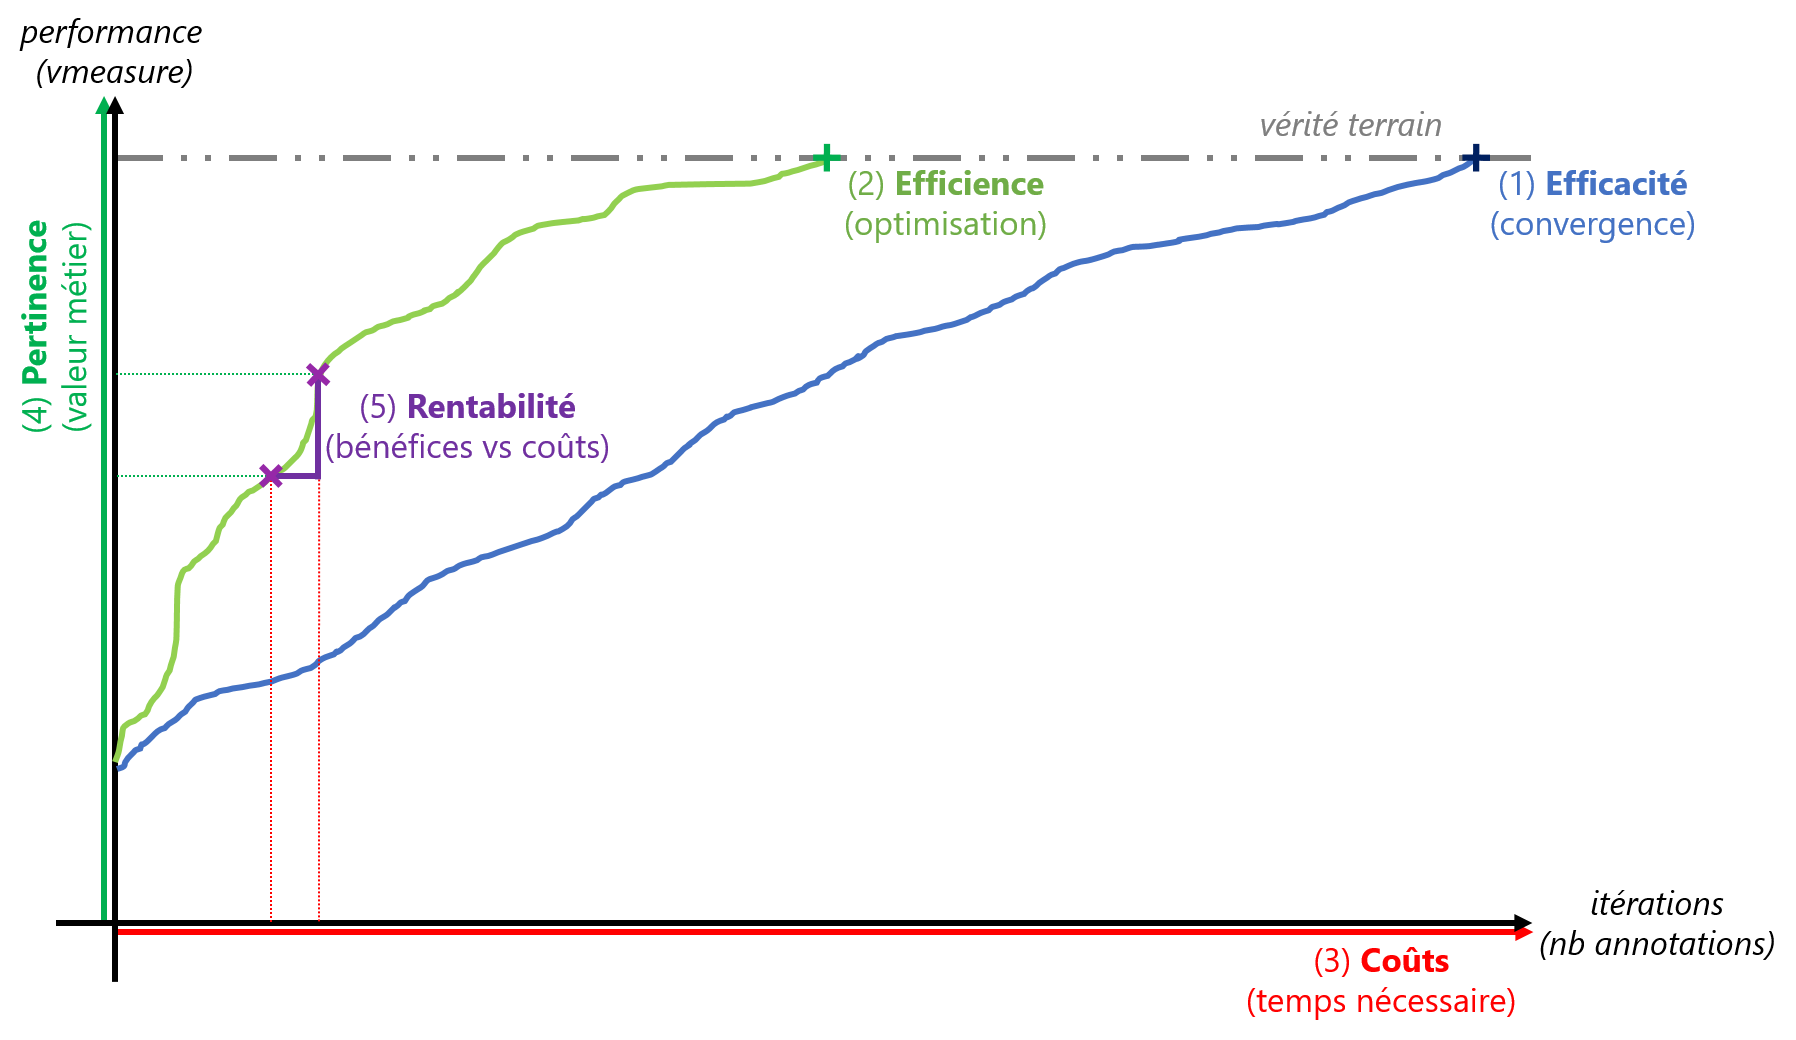
\includegraphics[width=0.95\textwidth]{figures/hypotheses-05-rentabilite}
			\caption{Illustration des études réalisées sur le \textit{clustering} interactif (\textit{étape 5/6}) en schématisant l'évolution de la pertinence (\textit{valeur métier évaluée par l'expert et exprimé en nombre de clusters}) d'une base d'apprentissage en cours de construction en fonction du coût temporel de la méthode (\textit{temps nécessaire à l'expert métier et à la machine}), ainsi que la rentabilité de chaque itération de la méthode (\textit{rapport entre le gain potentiel de pertinence et le coût à investir}).}
			\label{figure:4.5-HYPOTHESE-RENTABILITE}
		\end{figure}

	\end{tcolorbox}
		
	% Résumé de l'étude.
	Afin de vérifier cette hypothèse, nous explorons deux approches :
	\begin{itemize}
		\item l'évolution de l'\textbf{accord entre l'annotation de l'expert et le \textit{clustering}} sur lequel est basé l'échantillon d'annotation, permettant d'estimer si la machine doit encore être corrigée par l'annotateur  (cf. sous-section~\ref{section:4.5.1-ETUDE-RENTABILITE-ACCORD-ANNOTATION-CLUSTERING}) ;
		\item et l'évolution de la \textbf{différence entre deux \textit{clustering} successifs}, permettant de mesurer s'il y a eu des changements visibles dans le partitionnement des données après l'ajout des dernières contraintes (cf. sous-section~\ref{section:4.5.2-ETUDE-RENTABILITE-SIMILARITE-CLUSTERING}).
	\end{itemize}
	
	
	%%%
	%%% Subsection 4.5.1: Etude de l'accord entre annotation et \textit{clustering}
	%%%
	\subsection{Etude de l'accord entre annotation et \textit{clustering}}
	\label{section:4.5.1-ETUDE-RENTABILITE-ACCORD-ANNOTATION-CLUSTERING}
		
		% Objectif de l'expérience.
		\todo[inline]{A REDIGER: objectif de l'expérience}
	
		%%% Protocole expérimental.
		\subsubsection{Protocole expérimental}
			\todo[inline]{A REDIGER}
			% Axiome.
			% Pseudo-code.
			% Détails de l'expérience.
			
			
			% Référence scripts.
			\begin{leftBarInformation}
				Les scripts de l'expérience, réalisés avec des \textit{notebooks} Python (\cite{van-rossum-drake:2009:python-reference-manual}), sont disponibles dans un dossier dédié de~\cite{schild:2021:cognitivefactory-interactiveclusteringcomparativestudy}.
			\end{leftBarInformation}

		%%% Résultats
		\subsubsection{Résultats obtenus}
			\todo[inline]{A REDIGER}
		
			% Description statistiques.
			\todo[inline]{A REDIGER}
			
			% Figure.
			%
			\begin{figure}[!htb]
				\centering
				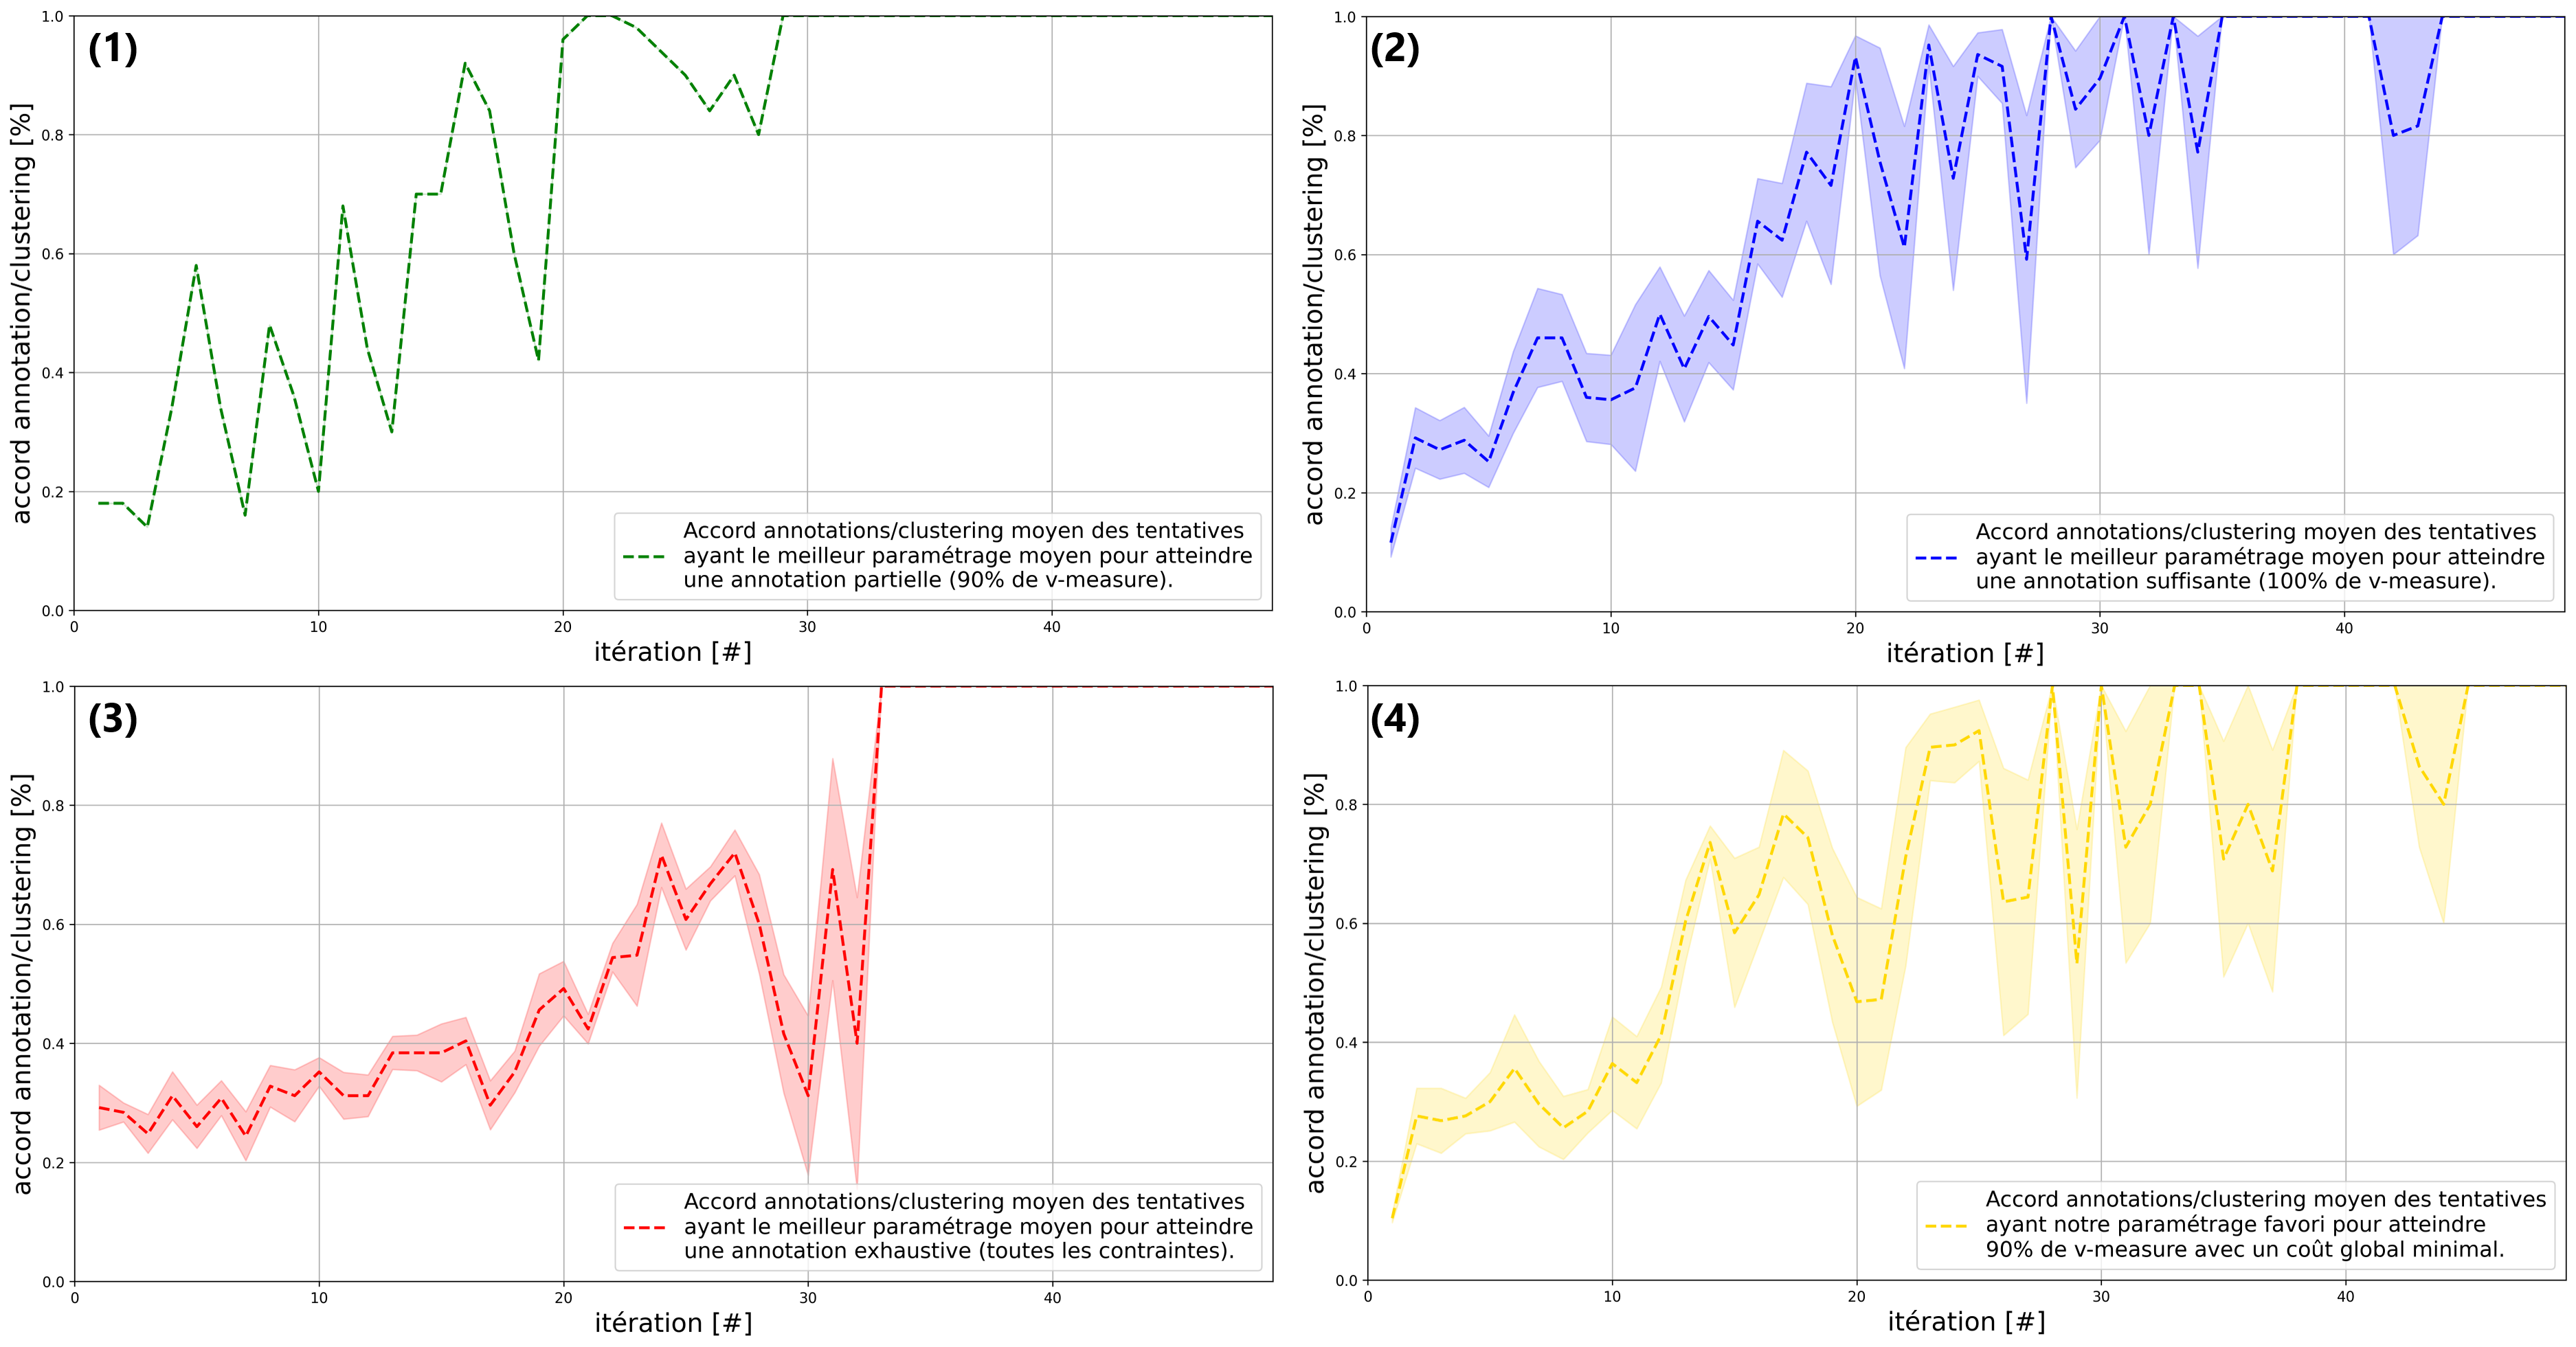
\includegraphics[width=0.95\textwidth]{figures/etude-rentabilite-accord-annotation}
				\caption{Évolution de l'accord entre annotation de contraintes d'un expert et le résultat de \textit{clustering} sur lequel est basé l'échantillonnage de contraintes.
				Les évolutions moyenne de différents paramétrages de la méthode sont exposées :
				\textbf{(1)} meilleur paramétrage moyen pour atteindre une annotation partielle ;
				\textbf{(2)} meilleur paramétrage moyen pour atteindre une annotation suffisante ;
				\textbf{(3)} meilleur paramétrage moyen pour atteindre une annotation exhaustive ;
				et \textbf{(4)} paramétrage favori.
				} 
				\label{figure:4.5.1-ETUDE-RENTABILITE-ACCORD-ANNOTATION-CLUSTERING}
			\end{figure}

		%%% Discussion
		\subsubsection{Discussion}
			\todo[inline]{A REDIGER}
		
			% Remaques.
			\todo[inline]{A REDIGER: C'est assez instable, cf. échantillonnage optomisé}
			
			% Conclusions et suggestion.
	
	
	
	%%%
	%%% Subsection 4.5.2: Etude de la différence de résultats de \textit{clustering} entre deux itérations
	%%%
	\subsection{Étude de la différence de résultats de \textit{clustering} entre deux itérations}
	\label{section:4.5.2-ETUDE-RENTABILITE-SIMILARITE-CLUSTERING}
		
		% Objectif de l'expérience.
		\todo[inline]{A REDIGER: objectif de l'expérience}
	
		%%% Protocole expérimental.
		\subsubsection{Protocole expérimental}
			\todo[inline]{A REDIGER}
			% Axiome.
			% Pseudo-code.
			% Détails de l'expérience.
			
			
			% Référence scripts.
			\begin{leftBarInformation}
				Les scripts de l'expérience, réalisés avec des \textit{notebooks} Python (\cite{van-rossum-drake:2009:python-reference-manual}), sont disponibles dans un dossier dédié de~\cite{schild:2021:cognitivefactory-interactiveclusteringcomparativestudy}.
			\end{leftBarInformation}

		%%% Résultats
		\subsubsection{Résultats obtenus}
			\todo[inline]{A REDIGER}
		
			% Description statistiques.
			\todo[inline]{A REDIGER}
			
			% Figure.
			%
			\begin{figure}[!htb]
				\centering
				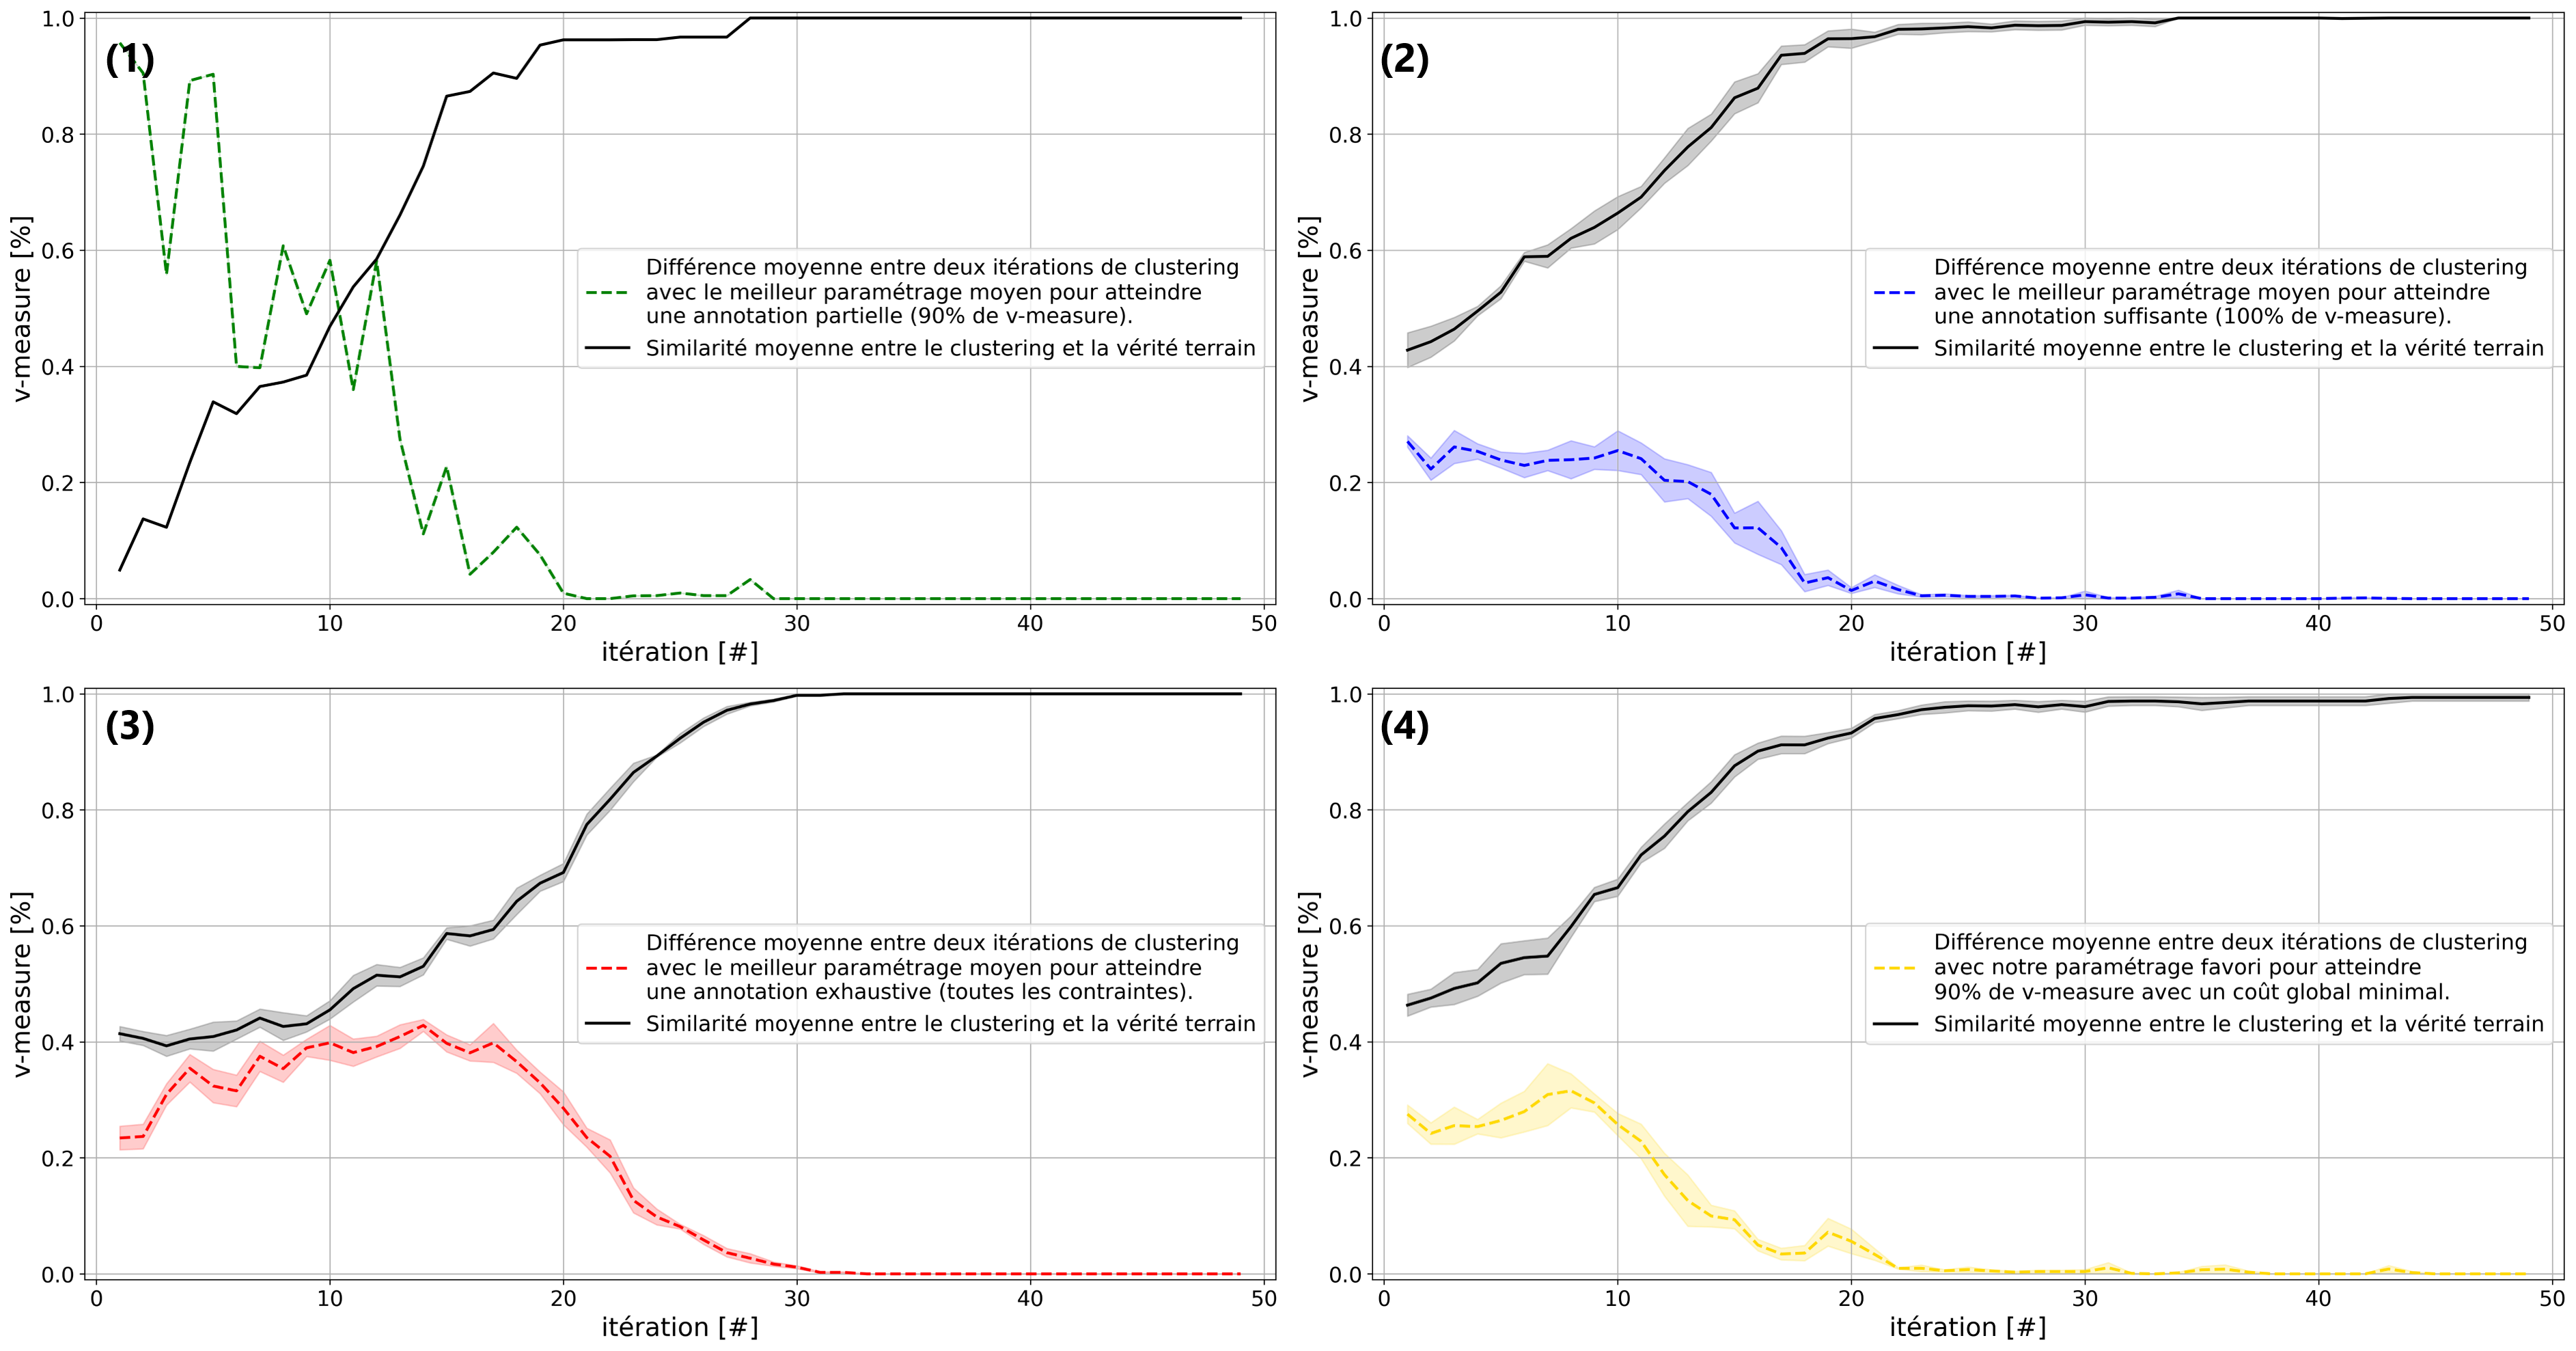
\includegraphics[width=0.95\textwidth]{figures/etude-rentabilite-similarite-clustering}
				\caption{Évolution de la différence de résultats entre deux itérations de \textit{clustering}.
				Les évolutions moyenne de différents paramétrages de la méthode sont exposées :
				\textbf{(1)} meilleur paramétrage moyen pour atteindre une annotation partielle ;
				\textbf{(2)} meilleur paramétrage moyen pour atteindre une annotation suffisante ;
				\textbf{(3)} meilleur paramétrage moyen pour atteindre une annotation exhaustive ;
				et \textbf{(4)} paramétrage favori.
				}
				\label{figure:4.5.2-ETUDE-RENTABILITE-SIMILARITE-CLUSTERING}
			\end{figure}

		%%% Discussion
		\subsubsection{Discussion}
			\todo[inline]{A REDIGER}
		
			% Remaques.
			\todo[inline]{A REDIGER: Ca montre quand plus rien bouge, fixer un seuil}
			
			% Conclusions et suggestion.